\section{Image Trasnformation Framework}
\label{sec:Pipeline}
%In this Section, we introduce our proposed pipeline to learn and generate beauty of urban images. 

%This section would introduce the process pipeline that we design to learn and generate urban images that enhance beauty in urban images drawn from street view. We do so by explaining individual components. The table \ref{notations} introduce the reader to the notations used. The block diagram \ref{fig:pipeline} shows the process stages. 
We present here a general algorithm for transforming natural geolocated images from one category to another. We will apply this algorithm for image beautificaiton in the next Section.
We summarise the notations used in Table \ref{notations} and the pipeline steps in Figure \ref{fig:pipeline}. 

\begin{table}[t]
  \resizebox{\linewidth}{!}{
  \begin{tabular}{l|p{8cm}}
    \textbf{symbol} & \textbf{stands for}\\
     $X$    & Georeferenced urban images data \\
     $I_i$    & Georeferenced image where $I_i \in X $ \\
     $Y$    & Annotations classes for $X$ in affective space ( We work with Beauty )\\
     $y_i$    & Annotation class in $Y$\\
     $\hat{I_j}$ & Template image \\
     $I'$ & Target Image \\
     $C$ & Image Classifier \\
     & \\
     \textbf{term} & \textbf{stands for}\\
     \textit{Template Image} $\hat{I_j}$    & A synthetic transformation of input image $I$ towards the class $y_j$ \\
     \textit{Target Image} $I'$    & The natural image which is most visually similar to the template image \\
    \textit{ Data Clustering}    & A process which groups images in $X$ according to visual similarity (e.g urban vs rural)\\
     \textit{Data Augmentation}    & A process which looks for images taken in the surrounding areas of the georeferenced images in $X$\\
     \textit{Classifier}   & A deep-learning framework that is able to classify images into one of the classes in $Y$\\
     \textit{Generator} $(GAN)$    & A deep-learning based generative framework to produce images similar to the ones in  $X$\\
     $DGN-AM$    & A framework that, given the GAN and the Classifier, transforms an input image into the template image.\\
            \end{tabular}}
  \caption{Notations and Terms.}\label{notations}
\end{table}

In general terms, the framework allows anyone with an arbitrary set of \emph{geolocated} images $ X = { I_1, I_2 ... . I_n  }$ annotated in classes $Y = {y_1 , y_2 , ... ,y_k}$, to transform natural images between classes: the algorithm can transform an  image $I_i$ belonging to class $y_i \in Y$ , to image $I_j$ from class $y_j \in Y$. Both $I_i$ and $I_j$ are natural, non-synthetic images. Despite having another \emph{meaning} (i.e. category), $I_j$ maintains the structural characteristics of $I_i$ (e.g. point of view, layout).  This allows  to visually reason about the discriminative properties between classes $y_i , y_j \in Y$, and visually understand the salient characteristics that drive a classifier to distinguish between  classes $y_i,y_j$. These questions might be trivial for tangible classes of objects \textbf{[ADD REFS]}, but still remain largely unexplored for intangible classes representing concepts like beauty, sentiment etc.  In this paper, we apply this general scheme to the specific problem of predicting and transforming beauty of urban images.

\par 
The transformation framework consists of three phases (see Fig. \ref{fig:pipeline}). The first phase %is a traditional image 
classifies images from $X$ into the corresponding categories $Y$ with high accuracy using a convolutional neural network $C$. %degree of precision.  
The second phase transforms am image from class $y_i$ to class $y_j$, using Generative Adversarial Networks (\textbf{[REF]}). The output of this phase is a synthetic image $\hat{I_j}$, which summarizes the basic traits of the destination class $y_j \in Y$. The last phase matches the synthetic image $\hat{I_j}$,  with the closest natural image in $X$.

%In the first phase, the pipeline simply learns the model of Beauty from the annotated data, such that it can classify Images from $X$ into classes $Y$ with high degree of precision. Assuming that the first phase builds a respectable model, the second phase is to transform images from class $y_i$ to class $y_j$. This done using Generative Adversarial Networks to produce prototype images or a template images $\hat{I_j}$, that represents the basic traits of the destination class $y_j \in Y$. The last step is to match this template image $\hat{I_j}$,  with the closest natural image in $X$.

%
 \begin{figure*}[ht]
	\centering
	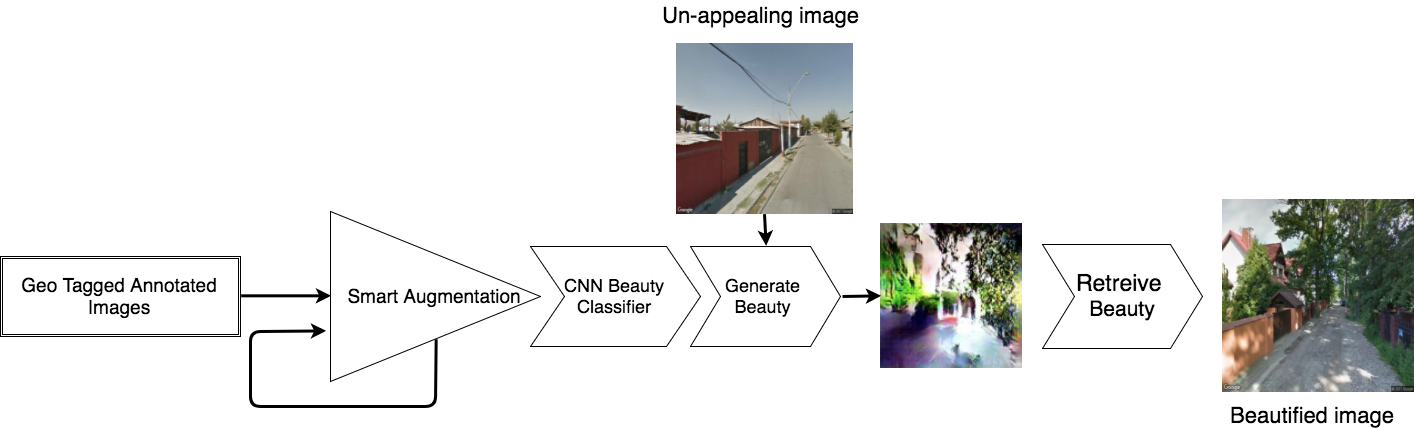
\includegraphics[width=2\columnwidth]{Plot/UrbanEmotionsPipeline.png}
	\caption{Architecture of the Beautification Pipeline}
    \label{fig:pipeline}
\end{figure*}

\subsection{Phase 1: Classifying Images}
We design here a classifier $C$  able to correctly assess the category $y_i$ of an image in $X$ using a deep learning network \textbf{[ADD REF ABOUT CNN REQUIRING A LOT OF DATA]}, we need first make sure we have enough reliable data to train the classifier. We do this by augmenting the available geolocated image data. 

%To increase that probability that a classifier $C$ is able to correctly assess the category $y_i$ of an image in $X$ using a deep learning network \textbf{[ADD REF ABOUT CNN REQUIRING A LOT OF DATA]}, we need first make sure we have enough reliable data to train the classifier. We do this by augmenting the available geolocated image data. 
%\subsubsection{Data Clustering}
%In urban images, the variance in structure and composition can be extremely high. 
%The main aim of data clustering is to reduce the diversity and variance in the image set. This is needed when working with  state of the art deep-learning classifiers, which generally work on highly specific classes of objects with low variance in the image semantics. %Two clustering methods are listed below.
%\textbf{[PLEASE LIST THE ONE YOU USED]}
%\begin{itemize}
%	\item The most simple yet effective way to cluster data %could be 
%	is based on geographical context. This can be done simply by using geographical boundaries of areas of interest and clustering images based on attributes like rural, urban, suburban, city etc.  This seems like an intuitive pre-processing step, as images from countryside look widely different compared to the images from the urban environment, and might be look visually diverse despite having similar annotations.
%	\item %
%	The other solution is to cluster images based on some visual/latent similarity measure. One possible way to do this is by extracting higher dimensional features, and clustering images based on these features.
%\end{itemize} 

 
\subsubsection{Data Augmentation}
%In the due process of clustering, it is expected that the total size of data available to train would reduce. 
Since smaller data size implies that a machine learning model has a risk of over-fitting,% and in the worst case not learning anything at all. Hence 
 we augment the data with some additional real and transformed data. Here, we take advantage of the geo-located nature of the images in our dataset. We also take advantage of the fact that some urban places in proximity, look quite similar to each other.  %Some of the techniques that may be used are listed below.
 \textbf{[AGAIN PLEASE LIST THE ONE YOU USED AND TALK ABOUT THE SMART AUG. \sj{IS it necessary now that we have a specific section for that ? }]}
\begin{itemize}
	\item The most common augmentation technique in deep learning literature is to do transformations on the image. Transformations like flipping images, cropping, adding noise , shifting color histograms can increase the data points for training and at the same time reduce the risks of over fitting. This technique however is not suitable for learning subjective urban qualities as the process may interfere with this very quality.
	\item Because the images are geo tagged, one can augment the data by acquiring additional images which fall very close geographically to the original image. In this approach, care must be taken to maintain visual similarity of additional images. Visual similarity can be ascertained in several ways including, but not limited to, using higher dimensional features extracted using some pre-trained image models, to measure image distance
\end{itemize}. 

\subsubsection{Classifier}
\label{sec:classifier}
Once we have enough data, we train a deep convolutional network so as to classify images into the $Y$ classes. One may use several successful deep convolutional neural network architectures, which work for other use cases like AlexNet \cite{krizhevsky2012imagenet} , PlacesNet \cite{zhou2014learning} or GoogLeNet \cite{szegedy2015going}.  For our paper we use CaffeNet which is a modified version of AlexNet. This trained classifier is a important component in the next phase, which is generation of images. 
%\textbf{[FEW WORDS ABOUT THE CLASSIFIER?]}

% In our case, we choose the classifier to be binary in nature because of the ranking distribution as seen in Fig \ref{fig:trueskill}. It is worth noting that the classification performance of this classifier would govern how articulately can you explain the network.

\subsection{Phase 2: Generating Images}
\par 
We now want to design a framework to transform any image $I$ into a template image $\hat{I_j}$ (as shown in Figure \ref{fig:pipeline}) %which is a synthetically perturbed version of $I$ such that it maximizes the activation for annotation class $y_j$. 
$\hat{I_j}$  is  a synthetic version of the original image, with added features and motifs that maximize class $y_j$. %The final step would transform this template image, into a natural image.
To produce the template image $\hat{I_j}$, we need the following components in place, 1) The classifier  $C$ which learns how to distinguish between different image categories $Y$ 2)  A generative model (GAN), that can generate samples from the distribution of the dataset images. 3) An activation maximization framework, that, based on the GAN generator, generates images that maximizes activation for a given annotation class \cite{dosovitskiy2016inverting} (our template images). 
\begin{itemize}
	\item{\textit{Classifier}}. %In order to produce template images, 
	To create synthetic representations of annotation classes, we first train the classifier $C$%deep learning based classifier,
	that, given an image $I$, can correctly classify it in one of $k$ classes. The aim of the rest of this pipeline is to explain \textit{what} the classifier is learning about the annotations. The assumption here is, once the classifier learns to discriminate amongst the classes, it also learns discriminative properties about the images that fall in those annotation categories. %Several works have shown that as a convolutional network trains, several semantic and object detectors emerge at higher abstraction levels in the network architecture. 
	
	\item \textit{Generator}. We train a generative adversarial network (GAN) which can generate an approximate natural looking image drawn from distribution of a particular class of images, similar to the one  in \cite{dosovitskiy2016inverting}. This GAN generator would learn to generate a natural-like image that represents the overall structure and knowledge about the Dataset.
	
	\item \textit{Activation Maximization}. We plug in the GAN and the classifier network into an Activation Maximisation (AM) framework. Given these components, an input image $I$, and a target class $y_i$, the AM transforms $I$ in an ideal image $\hat{I_j}$ ( that maximizes the activation for  class $y_i$). %The output of this step would be an image, which is very close to a natural image that the classifier is trained on, but has all the right motifs that maximizes the annotation class. 
	Essentially $\hat{I_j}$  is a representation of the overall knowledge about a particular annotation class, that the classifier network has learned through training. 
\end{itemize}	


\subsection{Phase 3: Retrieving Images }
In mathematical terms, we want to choose a target image $I'$ from $X$ so as to minimize $E(I' , \hat{I_j} )$ , where $E(I_1, I_2)$ is some error measure that quantifies visual error between two images. This image $I'$ is effectively a natural transformed image.
In this final step we find a target image $I'$ from the dataset that is closely aligned, in terms of some visual similarity metric $E(I_1, I_2)$, with the generated template image  $\hat{I_j}$ . The result of this exercise is to find the most similar looking image to an input image $I$ that maximizes a particular annotation class $y_j$.% So in a sense we are transforming one natural image into another natural image so as to maximize some annotation class. 
The visual differences in these two natural images, can act as the subject of reasoning for the explainability.